\newpage
\section{Causal Discovery using Order-Informed Context}

% SECTIONS
% LCD/ICP
% Design of context variables and justification of decisions
% Assumptions and justification
% Short validation of synthetic data



\subsection{Local Causal Discovery}

Local Causal Discovery has been proposed as a fast, incomplete algorithm to discover ancestral relations. The original formulation by \citet{cooper1997simple} depends on an underlying Bayesian Network and thus acyclicity. A more modern formulation by \citet{mooij2016joint} generalizes the algorithm to SCMs that allow cycles. 



\subsubsection{Assumptions}

The algorithm tests for a causal relation $X\to Y$ between two endogenous variables, using a third exogenous variable $C$ (the context). A small set of statistical independence tests restricts the set of possible causal subgraphs with $X$, $Y$ and $C$, and allowes us to infer under some circumstances that $X$ is an ancestor of $Y$. 

LCD is based on the following assumptions:

\begin{enumerate}
    \item Underlying SCM (JCI-0)
    \item Exogeneity of a context variable (JCI-1)
    \item Causal faithfulness
    \item Unbiased data selection
    \item Independence oracle, and Dependence oracle
\end{enumerate}



\subsubsection{Statistical tests}

LCD specifically discovers those causal relations, which effect can be measured from the data as $\Prb _M(Y|do(X=x)) = \Prb _M(Y|X=x)$. This is the case when only $X$ has an effect on $Y$ (i.e. no confounding or effect from $C$). Figure \ref{fig:5:lcdgraphs} shows the three subgraphs that satisfy this condition. Note that all possible relations between $C$ and $X$ given the exogeneity assumption are included.

All subgraphs satisfy one independence and five dependence relations:

\begin{enumerate}
    \item $C \CI Y \given X $
    \item $C \nCI X$
    \item $X \nCI Y$
    \item $C \nCI Y$ (follows from 2 and 3)
    \item $X \nCI Y \given C$ (follows from 1 and 3)
    \item $C \nCI X \given Y$ (follows from 1 and 2)
\end{enumerate}

The last three relations can be infered from the first three, using the causal faithfulness assumption and the Markov property. \citet{cooper1997simple} proved that the first three relations are sufficient to infer the causal relation $X\to Y$, by enlisting all possible subgraphs. 

Most LCD implementations only check the first three relations. However, if assumptions are violated, some nonexistent causal relations might be infered. One can sacrifice recall for precision by testing some or all of the last three relations. \citet{cooper1997simple} warns specifically that the independence relation ($C \CI Y \given X$) is vulnerable to faithfulness violations, and suggests testing the fourth relation ($C \nCI Y$) as well. \citet{triantafillou2017predicting} aim for high precision and test all six relations.

A common choice of dependence test is the two-tailed Fisher z-test \citep{fisher1924distribution}, which tests if the partial correlation is zero. Specifically, if we want to test $X \nCI Y \given Z$, we set the hypotheses:

\begin{itemize}
    \item[$H_0$:] $\rho_{XY|Z}=0$
    \item[$H_A$:] $\rho_{XY|Z}\not = 0$
\end{itemize}

The partial correlation 

z-transform -> test statistic z

test hypothesis: p = 2*PHI(-sqrt... |z|)

Pragmatic: use as independence test as well (different alpha, usually same value, but e.g. not in \citet{triantafillou2017predicting})


SOMETHING ABOUT ASYMMETRY, but what was it and where did I read it?




\begin{figure}[]
    \centering
    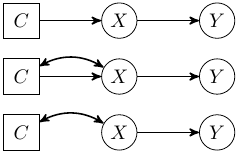
\includegraphics[width=.3\textwidth]{5LCDgraphs.png}
    \caption{Subgraphs in which LCD infers $X\to Y$}
    \label{fig:5:lcdgraphs}
\end{figure}